\documentclass{article}
\usepackage[capitalise]{cleveref}
\usepackage[UKenglish]{babel}
\usepackage[UKenglish]{isodate}
\usepackage[utf8]{inputenc}
\usepackage{microtype}
\usepackage{tikz}
\usepackage{amsfonts}
\usepackage[affil-it]{authblk}

\usetikzlibrary{arrows}
\usetikzlibrary{arrows.meta}
\usetikzlibrary{shapes}

\usepackage{natbib}
\bibliographystyle{abbrvnat}

\title{Recursive Solutions to First-Order Model Counting}
\author{Paulius Dilkas}
\author{Vaishak Belle}
\affil{University of Edinburgh, Edinburgh, UK}

\begin{document}
\maketitle

% Definition and scope of the topic: FOMC

\emph{First-order model counting} (FOMC) is the problem of computing the number of models of a sentence in first-order logic given the size(s) of its domain(s) \citep{DBLP:conf/ijcai/BroeckTMDR11}. The main application of FOMC (or, rather, its \emph{weighted} variant WFOMC) is in probabilistic inference, particularly for statistical relational models such as Markov logic networks that define probabilities over sets of objects and relations thereof \citep{DBLP:conf/ijcai/BroeckTMDR11,DBLP:journals/cacm/GogateD16}.

Over slightly more than a decade, research on (W)FOMC advanced on both theoretical and empirical fronts. Several WFOMC algorithms such as ForcLift \citep{DBLP:conf/ijcai/BroeckTMDR11}, probabilistic theorem proving \citep{DBLP:journals/cacm/GogateD16}, and L2C \citep{DBLP:conf/kr/KazemiP16} were developed. More and more classes of formulas were shown to be \emph{liftable}, i.e., solvable in polynomial time with respect to the size(s) of the domain(s) \citep{DBLP:conf/kr/BremenK21,DBLP:conf/nips/KazemiKBP16,DBLP:conf/lics/KuusistoL18,DBLP:journals/jair/Kuzelka21}. Much of the researchers' attention was devoted to developing efficient solutions to formulas with up to two variables \citep{DBLP:conf/uai/BremenK21,DBLP:journals/corr/abs-2110-05992}.

% The problem you are to focus on the topic: recursion

However, none of the publicly available (W)FOMC algorithms can efficiently compute functions as simple as a factorial.\footnote{The problem of computing the factorial can be described using two variables and counting quantifiers, so it belongs to a fragment of first-order logic which is known to be liftable \citep{DBLP:journals/jair/Kuzelka21}.} We claim that this shortcoming is due to the inability of these algorithms to construct recursive solutions.

% If the problem was faced before, describe the state of the art.

The topic of recursion in the context of WFOMC has been studied before but in very limited ways. \Citet{DBLP:conf/ilp/BarvinekB0ZK21} use WFOMC to generate numerical data which is then used to conjecture recurrence relations that explain that data. \Citet{DBLP:conf/nips/Broeck11} introduced the idea of \emph{domain recursion}. Intuitively, domain recursion partitions a domain of size $n$ into a single explicitly named constant and the remaining domain of size $n-1$. However, many stringent conditions are enforced to ensure that the search for a tractable solution always terminates.

%1) But their code only conjectures stuff on data. My conjectures are guaranteed always true.
%2) everything has to be expressible in $\mathbf{C}^2$, i.e., the two-variable fragment of first-order logic with counting quantifiers on one domain.
%3) They only consider P-recursive functions, which means that, e.g., $f(n) = f(n-1)f(n-2)$ would not be allowed.

% Discuss the methods and novel techniques to be employed

\begin{figure}[t]
  \centering
  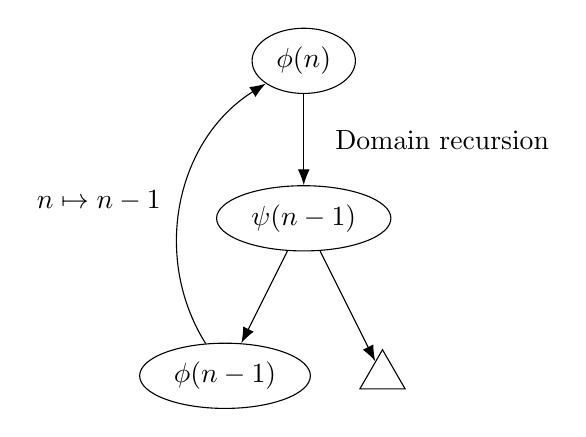
\begin{tikzpicture}[triangle/.style = {regular polygon, regular polygon sides=3}]
    \node[draw,ellipse] (a) at (0, 0) {$\phi(n)$};
    \node[draw,ellipse] (b) at (0, -2) {$\psi(n-1)$};
    \node[draw,ellipse] (c) at (-1, -4) {$\phi(n-1)$};
    \node[draw,triangle] (d) at (1, -4) {};
    \draw[-{Latex[length=2mm]}] (a) -- (b) node [midway,xshift=50] {Domain recursion};
    \draw[-{Latex[length=2mm]}] (b) -- (c);
    \draw[-{Latex[length=2mm]}] (b) -- (d);
    \draw[-{Latex[length=2mm]}] (c) to [bend left=45] node [midway,xshift=-30] () {$n \mapsto n-1$} (a);
  \end{tikzpicture}
  \caption{A conceptual illustration of the main idea}
  \label{fig:idea}
\end{figure}

In this work, we show how new tractable solutions can be found by dispensing with these restrictions. With additional compilation rules and an algorithm for checking whether a `recursive call' is possible, ForcLift \citep{DBLP:conf/ijcai/BroeckTMDR11} can construct recursive functions that efficiently solve counting problems that used to be beyond its reach. The main conceptual difference from the original algorithm is that the input formula is now compiled to a labelled directed graph rather than a circuit (i.e., cycles are allowed). This idea is illustrated in \cref{fig:idea}. Suppose the original formula $\phi$ depended on a domain of size $n \in \mathbb{N}$. Domain recursion transforms $\phi$ into a different formula $\psi$ that depends on a domain of size $n-1$. After some number of subsequent transformations, the algorithm identifies that a solution to $\psi$ can be constructed in part by finding a solution to a version of $\phi$ where the domain of size $n$ is replaced by a domain of size $n-1$. Recognising $\phi$ from before, we can add a cycle-forming edge to the graph, which can be interpreted as function $f$ relying on $f(n-1)$ to compute $f(n)$.

%% \begin{itemize}
%% \item one can then extract the (potentially recursive) definitions of functions from the graph
%% \item simplify the algebraic expressions, e.g.:
%%   \begin{itemize}
%%   \item adding and subtracting the same thing
%%   \item $\sum_{i=0}^n[i < 2]f(i) = f(0) + f(1)$
%%   \end{itemize}
%% \item evaluate the functions
%% \item definition of an FCG
%% \item maybe example of an FCG for injections
%% \item new compilation rules
%%   \begin{itemize}
%%   \item (generalised) domain recursion (via example)
%%   \item constraint removal (via example)
%%   \item recursion checking algorithm (sketch it)
%%   \end{itemize}
%% \item combining BFS and greedy search
%% \item smoothing needs to be adapted so as to not get stuck in an infinite loop
%% \item dynamic programming may be necessary to compute in polynomial time
%% \end{itemize}

% Highlights of the results obtained

In our experiments, we consider variations of the function-counting problem. These functions vary in:
\begin{itemize}
\item whether they are full or partial,
\item whether they are injective/surjective/bijective or not,
\item and whether the domain and the codomain are the same.
\end{itemize}
Many versions of this problem were previously unsolvable by any available (W)FOMC algorithm, whereas we can find recursive solutions (that can be evaluated in polynomial time) to all except one of these problems.

%% \begin{itemize}
%% \item $\Theta(mn)$ for $[m] \to [n]$ injections (optimal: $\Theta(\log m)$)
%% \item $\Theta(m)$ for $[m] \to [n]$ bijections (optimal: $\Theta(\log m)$)
%% \item TODO: add/explain the formulas as well
%% \end{itemize}

% Possible future enhancements and further work in progress

Further work is necessary to fully automate this new way of computing the (W)FOMC of a formula. The new version of ForcLift produces a graph which then needs to be transformed to definitions of (potentially recursive) functions. In some cases, it is necessary to simplify the algebraic expressions in these definitions (e.g., reducing $x-x$ to zero for some expression $x$). Most importantly, the algorithm only gives us the recursive calls but not the base cases. What makes the problem of finding these base cases non-trivial is that the number of base cases is not constant for functions of arity greater than one (i.e., formulas that mention more than one domain). Nonetheless, these remaining challenges are minuscule compared to the broader goal of expanding the capabilities of (W)FOMC to new classes of instances.

%% \begin{itemize}
%% \item open questions:
%%   \begin{itemize}
%%     \item what kind of sequences are computable in this way?
%%     \item would using a different logic extend the capabilities of FOMC even further?
%%   \end{itemize}
%% \end{itemize}

\bibliography{extended_abstract}

\end{document}
